\documentclass[oneside]{article}
\usepackage[latin1]{inputenc}
\usepackage[brazil]{babel}
\usepackage{graphicx}
\usepackage{listings}
\usepackage{xcolor}
\usepackage{amsmath}
\usepackage{hyperref}
\usepackage{url}
\usepackage{breakurl}
\usepackage[left=2.7cm, right=2.7cm, bottom=3cm]{geometry}
\usepackage{caption}
\usepackage{subcaption}
\usepackage{lipsum}
\usepackage{fancyhdr}
\usepackage{listing}
\usepackage{gensymb}

%\renewcommand*{\refname}{Refer�ncias Bibliogr�ficas}

\fancyfoot[c]{\thepage}
\fancyhead[ro,le]{}
\fancyhead[lo]{\leftmark}
\fancyhead[re]{\rightmark}

\lstset{%
	linewidth=\textwidth,%framed box is the text size 
	xleftmargin=.25in,
	xrightmargin=.25in, 
	frame=trbl, 
	columns=flexible, 
	captionpos=t, 
	upquote=false,
	basicstyle=\small\ttfamily,
	firstnumber=1,% 
	numberfirstline=false,% 
	numbers=left,%
	numberstyle=\tiny,% 
	stepnumber=5,%
	numbersep=5pt,% 
	backgroundcolor=\color{green!15},% 
	tabsize=4,% 
	keywordstyle=\color{green!65!black},% 
	commentstyle=\color{blue},% 
	stringstyle=\color{magenta},% 
	breaklines=true,% 
	emph={label},%
	abovecaptionskip=10pt,% 
	belowcaptionskip={\abovecaptionskip},%
	showstringspaces=false, 
	literate={�}{{\^{E}}}1
}%

\lstdefinestyle{code} {%
	basicstyle=\ttfamily\footnotesize,
	backgroundcolor=\color{blue!10},
	%escapeinside={@}{@},
	frame=single, 
	captionpos=t,
	upquote=false,
	numberfirstline=false,% 
	stepnumber=5,%
	tabsize=4,% 
	keywordstyle=\color{green!65!black},% 
	commentstyle=\color{blue},%
	stringstyle=\color{magenta},% 
	breaklines=true,% 
	emph={label},%
	abovecaptionskip=10pt,% 
	belowcaptionskip={\abovecaptionskip},%
}%

\title{
	\vspace{40pt}
	Uso de Reconhecedor e Sintetizador de Voz Embarcados para Controle de Equipamentos Eletr�nicos via Luz Infravermelha
	% Controle de Aparelhos Eletr�nicos por Sistemas Embarcados com Suporte � Reconhecimento e S�ntese de Voz
	\vspace{25pt}
}

\author{
	Cassio Trindade Batista\\
	\texttt{cassio.batista.13@gmail.com}\\
	\texttt{201106840003}
	\and
	Gabriel Peixoto de Carvalho\\
	\texttt{gaburiero.c@gmail.com}\\
	\texttt{201106840010}
	\and
	Pedro Henrique C. F. Soares\\
	\texttt{pedrofigueiredoc@gmail.com}\\
	\texttt{201106840007}
	\and
	Thiago Barros Coelho\\
	\texttt{tbarroscoelho@gmail.com}\\
	\texttt{201106840041}
}

\date{
\vspace{100pt}
\begin{table}[!h]
	\begin{tabular*}{.9\linewidth}{p{.45\linewidth}p{.45\linewidth}}
	& Projeto apresentado � disciplina Projetos de \textit{Hardware} e Interfaceamento 
	como requisito de avalia��o.
	Professores: Jeferson Breno N. Leite e Adalbery Rodrigues Castro.
	\end{tabular*}
\end{table}
\vfill
Belem -- Brasil\\
\vspace{2pt}
Maio/2015
}

\begin{document}
% capa ------------------------------------------------------------------------
\thispagestyle{empty}
\begin{center}
\includegraphics[width=.16\textwidth]{Figures/logo_ufpa}\\

\vspace{12pt}
\bf\large
UNIVERSIDADE FEDERAL DO PAR�\\\vspace{1.5pt}
INSTITUTO DE TECNOLOGIA\\\vspace{1pt}
FACULDADE DE ENGENHARIA DA COMPUTA��O E\\\vspace{1.5pt}
TELECOMUNICA��ES\\

\vspace{120pt}
{\Large
Uso de Reconhecedor e Sintetizador de Voz Embarcados para Controle de Equipamentos Eletr�nicos via Luz Infravermelha\\
%Controle de Aparelhos Eletr�nicos por Sistemas Embarcados com Suporte � Reconhecimento e S�ntese de Voz\\
}

\vfill
\normalsize
Bel�m -- Brasil\\
Junho/2015
\end{center}
%%% EOF %%%


% T�tulo e Pre�mbulo -----------------------------------------------------------
\newpage
\maketitle
\thispagestyle{empty}

% Sum�rio e Lista de Figuras ---------------------------------------------------
\newpage
\tableofcontents
\listoffigures

%% Lista de Abreviaturas --------------------------------------------------------
%\newpage
%\begin{section}{Lista de Abreviaturas}
%\begin{description}
%	\item[AM] \textit{Acoustic Model}
%	\item[ARPA] U.S. \textit{Department of Defense Advanced Research Project Agency}
%	\item[ASR] \emph{Automatic Speech Recognition} 
%	\item[API] \emph{Application Programming Interface}
%	\item[BSD] \textit{Berkeley Software Distribution} 
%	\item[CLI] \textit{Common Language Infrastructure} 
%	\item[CLR] \textit{Common Language Runtime}
%	\item[CNPq] Conselho Nacional de Desenvolvimento Cient�fico e Tecnol�gico
%	\item[FISL] F�rum Internacional de Software Livre
%	\item[HMM] \textit{Hidden Markov Model}
%	\item[HTK] \emph{Hidden Markov Model Toolkit}
%	\item[IBGE] Instituto Brasileiro de Geografia Estat�stica
%	\item[IEEE] \textit{Institute of Electrical and Electronics Engineers} 
%	\item[IR] \textit{Infra Red}
%	\item[JSAPI] \emph{Java Speech Programming Interface}
%	\item[JSGF] \textit{Java Speech Grammar Format}
%	\item[LM] \textit{Language Model}
%	\item[LVCSR] \textit{Large Vocabulary Continuous Speech Recognition} 
%	\item[MAP] \textit{Maximum A Posteriori} 
%	\item[MFCC] \textit{Mel-Frequency Cepstral Coefficients} 
%	\item[MLLR] \textit{Maximum Likelihood Linear Regression}
%	\item[NLP] \textit{Natural Language Processing}
%	\item[PT\_BR] Portugu�s Brasileiro 
%	\item[xRT] \textit{Real-time factor} 
%	\item[SAPI] \emph{Speech Application Programming Interface}
%	\item[SDK] \textit{Software Development Kit} 
%	\item[SR] \textit{Speech Recognition}
%	\item[TTS] \textit{Text to Speech} 
%	\item[UFPA] Universidade Federal do Par� 
%	\item[URL] \textit{Unified Resource Locator} 
%	\item[WER] \textit{Word Error Rate}
%	\item[XML] \textit{Extensible Markup Language}
%\end{description}
%\end{section}

% Introdu��o -------------------------------------------------------------------
\newpage
\pagestyle{fancy}
\begin{section}{Introdu��o}
A interface homem-m�quina encontra-se cada vez mais amig�vel. O que antes era
portado somente por empresas e pessoas com poder financeiro diferenciado e acima
da m�dia, em termos de tecnologia, � hoje muito mais acess�vel e simples para
usu�rios dom�sticos sem profundo conhecimento no assunto. Devido a abrang�ncia 
de computadores pessoais e embarcados e da Internet, novas oportunidades 
e expectativas em termos de trabalho, estudos e at� lazer s�o criadas a fim de 
melhorar ainda mais essa comunica��o, de modo que a m�quina se aproxime mais de
a��es t�picas do ser humano, como pensar e falar.

Acredita-se que a s�ntese e o reconhecimento autom�tico de voz (do ingl�s
\textit{text-to-speech} e \textit{automatic speech recognition},
respectivamente, TTS e ASR)~\cite{Taylor09,Huang01} tornam a interface citada
acima muito mais pr�tica e natural, de forma que a comunica��o de fato se
assemelha �quela estabelecida entre duas pessoas. O ASR refere-se ao sistema
que, tomando o sinal de fala digitalizado como entrada, � capaz de gerar o texto
transcrito na sa�da. J� um sistema TTS realiza a fun��o contr�ria, na qual um
sinal anal�gico de voz � sintetizado de acordo com o texto posto na entrada. 
Dentre as in�meras aplica��es que utilizam os sistemas que envolvem 
processamento de fala, pode-se destacar a automa��o residencial que visa ajudar
pessoas que tenham dificuldades no controle de alguns equipamentos eletr�nicos,
dando �nfase � acessibilidade alcan�ada atrav�s das tecnologias assistivas.

% Components of Quality of Life for Persons With a Quadriplegic and Paraplegic Spinal Cord Injury
Tecnologia Assistiva (TA) � um campo da engenharia biom�dica dedicada � aumentar
a independ�ncia e mobilidade de pessoas com defici�ncia, englobando
metodologias, pr�ticas e servi�os que objetivam promover sua autonomia,
qualidade de vida e inclus�o social~\cite{cat,Gelderblom02}. Tal tecnologia busca
reduzir a necessidade vivenciada por pessoas que precisam de solu��es que n�o as
deixem � margem da utiliza��o de dispositivos eletr�nicos.  Em outras palavras,
para diminuir a exclus�o digital imposta pela incapacidade de manipular certos
dispositivos, a acessibilidade � vista como elemento fundamental para elevar a
autoestima e o grau de independ�ncia dessas pessoas. Al�m disso, as mesmas
solu��es apresentadas podem ser �teis tamb�m para os n�o portadoras de
necessidades especiais, j� que o controle de equipamentos se torna mais pr�tico
e confort�vel.

Nesse sentido, este trabalho busca preparar um servidor local port�til de
reconhecimento e s�ntese de voz em Portugu�s Brasileiro (PT\_BR) baseado no
microcomputador BeagleBone Black de modo que, quando acessado pelo dispositivo
que agir� como controle remoto --- no caso, um smartphone com sistema
operacional Android ---, seja capaz de acessar as fun��es mais b�sicas de um
aparelho televisivo. Vale ressaltar que todas as APIs, IDEs, \textit{softwares},
bibliotecas e pacotes utilizados para cria��o dos sistemas e dos recursos
utilizados possuem licen�a \textit{open source} e s�o encontrados dispon�veis
livremente na Internet.
\end{section}
%%% EOF %%%


% Objetivos --------------------------------------------------------------------
\begin{section}{Objetivos}
O objetivo principal consiste em criar um prot�tipo port�vel, baseado em um
microcomputador embarcado, que seja capaz de controlar um aparelho de televis�o
atrav�s do envio remoto de sinais. O sistema ser� configurado como um servidor
que disponibiliza um servi�o gen�rico de reconhecimento de fala, de modo que o
aparelho de TV mencionado possa ser remotamente controlado atrav�s da voz do
usu�rio; e um servi�o de s�ntese de fala, provendo \textit{feedback} das a��es
de acordo com o entendimento do sistema de ASR. 
Al�m disso, a informa��o a ser enviada para a TV deve ser armazenada em um banco
de dados, tamb�m configurado no mesmo servidor.

\begin{figure}
	\centering
	\includegraphics[width=.80\textwidth]{Figures/schematic}
	\caption{Esquem�tico do Projeto.}
	\label{fig:sch}
\end{figure}

\subsection{Reconhecimento e S�ntese de Voz}
Para que o reconhecimento autom�tico de voz seja poss�vel, o \textit{software}
Julius dever� ser instalado no servidor. Julius � um software capaz de processar
e decodificar �udio em aproximadamente tempo real para tarefas de ditado de at�
60 mil palavras. Este tamb�m ser� o principal programa do sistema, o qual
receber� em seu c�digo nativo todos os outros m�dulos.

Para que o Julius possa realizar o reconhecimento em Portugu�s Brasileiro, ser�o
necess�rios basicamente dois recursos: um modelo ac�stico e um dicion�rio
fon�tico. Modelos ac�sticos gen�ricos para PT\_BR podem ser encontrados na
p�gina do Grupo FalaBrasil~\cite{falabrasilsite}, bem como o software que cria o
dicion�rio fon�tico (conversor grafema-fonema ou G2P)~\cite{Siravenha08}.
Entretanto, embora a taxa de acerto dos modelos seja satisfat�ria, ainda h�
casos nos quais a acur�cia do modelo n�o � suficiente. Nesse caso, � poss�vel
melhor�-la atrav�s da cria��o ou treino de modelos espec�ficos para a aplica��o.
O processo de treino � realizado pelo software HTK (\textit{Hidden 
Markov Models Toolkit}), o qual � capaz de extrair segmentos de fala de um
arquivo de �udio e assinalar uma refer�ncia � ele. Tal refer�ncia � retirada do
dicion�rio fon�tico, previamente criado com o software G2P.

O software eSpeak � a principal refer�ncia em s�ntese de voz em ambientes Linux.
Gra�as � disponibiliza��o de uma API no site oficial do desenvolvedor,
o sistema, al�m de conseguir ``ouvir e entender'', tamb�m ser� capaz de 
``falar''. O download dos modelos para PT\_BR � feito juntamente com o das
bibliotecas necess�rias. Como a BBB n�o possui sa�da de �udio nativa, um
auto-falante USB ser� utilizado.

\subsection{Controle Remoto de TV e Servidor LAMP}
Os aparelhos televisivos atuais, assim como a grande maioria dos dispositivos
eletr�nicos dom�sticos, possuem a tecnologia de controle remoto baseada em luz
infravermelha. Pode-se observar que na extremidade superior dos controles
remotos, h� pelo menos um led infravermelho (IR Led) capaz de emitir luz e,
dessa forma, transmitir uma informa��o bin�ria para o circuito localizado na 
parte frontal da TV. Esse circuito possui um sensor infravermelho (IR sensor), o
qual, atuando como o receptor da comunica��o, � capaz de receber os bits
transmitidos e repass�-los para o processador do circuito, o qual executar� a
tarefa relacionada � decodifica��o dos bits (desligar a TV, mostrar o menu,
etc).

Nesse sentido, um m�dulo receptor ser� adicionado � BeagleBone para que esta
seja capaz de ``hackear'', atrav�s de um sensor infravermelho, informa��es dos
controles remotos, dado que o acesso aos \textit{datasheets} de diversos
aparelhos n�o � trivial.  O sistema de gerenciamento de banco de dados MySQL
ser� instalado e configurado no servidor para armazenar o c�digo, o qual �
relacionado a a��es como ``aumentar volume'' ou ``desligar'' da TV principal e
dos demais aparelhos que vierem a ser cadastrados no banco.  Toda a informa��o
de sa�da a ser enviada para a TV atrav�s dos IR leds deve ser oriunda do banco
de dados. 
% Al�m disso, bibliotecas que permitem o acesso ao MySQL por c�digos em
% C ser�o instaladas, j� que essa � a principal linguagem do software do servidor.
\end{section}
%%% EOF %%%


% Justificativa ----------------------------------------------------------------
\begin{section}{Justificativa}
% [IBGE'10] ftp://ftp.ibge.gov.br/Censos/Censo_Demografico_2010/Caracteristicas_Gerais_Religiao_Deficiencia/tab1_3.pdf
% http://g1.globo.com/brasil/noticia/2012/04/239-dos-brasileiros-declaram-ter-alguma-deficiencia-diz-ibge.html
Segundo o Instituto Brasileiro de Geografia e Estat�stica (IBGE), no censo
realizado em 2010, aproximadamente 23,9\% dos brasileiros declaram ter alguma
defici�ncia~\cite{ibge10}. Esse n�mero ainda � mais impressionante quando se
pensa que cerca de um quarto de uma popula��o de 190 milh�es de habitantes �
portadora de alguma necessidade especial. Ainda segundo os dados, 6,9\%
(13,3~mi) dos brasileiros apresentam algum grau de defici�ncia motora, enquanto
18,8\% (35,7~mi) afirmam serem cegas ou terem alguma dificuldade para enxergar.

Essa pesquisa tem como finalidade apresentar uma solu��o para diminuir a
exclus�o digital vivenciada especialmente por pessoas com necessidade motora ou
visual, as quais est�o � margem da utiliza��o de dispositivos eletr�nicos
por conta da aus�ncia se solu��es que os adaptem �s suas necessidades. A
tecnologia de reconhecimento de fala torna acess�vel a utiliza��o de qualquer
dispositivo eletr�nico por usu�rios incapazes de realizar movimentos espec�ficos
com membros superiores, como segurar um controle f�sico e apertar bot�es ou
digitar, por exemplo. Al�m disso, os portadores de necessidades visuais tamb�m
poder�o ser ajudados, j� que nem todos os controles possuem refer�ncias
reconhec�veis pelo tato. A s�ntese de fala tamb�m se torna muito importante no
contexto da dificuldade visual, j� que um \textit{feedback} via texto, nesse
sentido, seria pouco �til.

% Ref.: ADA - American with Disabilities Act
O Ato de Americanos com Defici�ncia (ADA)~\cite{ada} � um documento que regula
os direitos dos cidad�os com defici�ncia nos EUA, al�m de prover a base legal
dos fundos p�blicos para compra dos recursos que estes necessitam. Algumas
categorias de TA foram criadas com base nas diretrizes gerais da ADA, das quais
podemos salientar tr�s como justificativa do trabalho:

\begin{enumerate}
	\item Recursos de acessibilidade ao computador
	\begin{itemize}
		\item Equipamentos de entrada e sa�da (\underline{s�ntese de voz}, 
		Braille), aux�lios alternativos de acesso (ponteiras de cabe�a, de luz),
		teclados modificados, softwares especiais (\underline{reconhecimento de 
		voz}, etc.), que permitem as pessoas com defici�ncia a usarem o 
		computador.
	\end{itemize}
	\item Sistemas de controle de ambiente
	\begin{itemize}
		\item Sistemas eletr�nicos que permitem as pessoas com limita��es
		moto-locomotoras controlar remotamente aparelhos eletro-eletr�nicos,
		sistemas de seguran�a, entre outros, localizados em seu quarto, sala,
		escrit�rio, casa e arredores.
	\end{itemize}
	\item Aux�lios para cegos ou com vis�o subnormal
	\begin{itemize}
		\item Aux�lios para grupos espec�ficos que inclui lupas e lentes,
		Braille para equipamentos com \underline{s�ntese de voz}, grandes telas 
		de impress�o, sistema de TV com aumento para leitura de documentos, 
		publica��es etc.
	\end{itemize}
\end{enumerate}

A decis�o de criar um servidor pr�prio de s�ntese e reconhecimento de voz
baseia-se principalmente na possibilidade de usufruir de tais recursos de forma
offline, ou seja, sem a necessidade de conex�o com a Internet. No caso do
sistema ASR, pode-se tamb�m citar a vantagem de limitar o vocabul�rio de
palavras utilizados atrav�s da implementa��o de uma gram�tica, j� que servi�os
online de reconhecimento (como o disponibilizado pelo Google, por exemplo),
trabalham com a inteira modelagem das palavras do idioma, impossibilitando a
cria��o de um contexto espec�fico para a aplica��o. Al�m disso, o uso de APIs
externas n�o resulta no aprendizado sobre a filosofia do reconhecimento de fala,
o que tornaria o trabalho menos interessante.

\textcolor{red}{*Add some conclusion to the section here*}
\end{section}


% Revis�o Te�rica --------------------------------------------------------------
\begin{section}{Revis�o Te�rica}
% [IEEE'11] Designing Android Applications with both Online and Offline Voice Control of Household Devices
% [IEEE'10] Smart Home Control System for the disabled using the head and the mouth movement
% [IJERA'15] Wi-Fi and Android Based Smart Home Automation for People with Disabilities
 
Como o iOS e o Android foram lan�ados, respectivamente, em 2007 e 2008, e 
a ascens�o dos smartphones � relativamente recente, a ideia de aplicar
acessibilidade no controle de equipamentos eletr�nicos atrav�s desse tipo de
equipamento somente come�ou a revelar resultados concretos a partir de 2010. 
Em~\cite{ieee11}, o decodificador PocketSphinx foi embarcado em um smartphone
android para que este pudesse controlar aparelhos dom�sticos atrav�s da
interface de voz. O resultado era enviado para uma SparkFun IOIO Board, a qual
disparava o \textit{trigger} para o controle de uma TV. O foco do trabalho era
ajudar pessoas afetadas com tetraplegia a serem mais independentes, al�m de
avaliar o desempenho de decodificadores embarcados e distribu�dos, claro.

\textcolor{red}{*Add another reference here*}

\begin{figure}[!h]
	\centering
	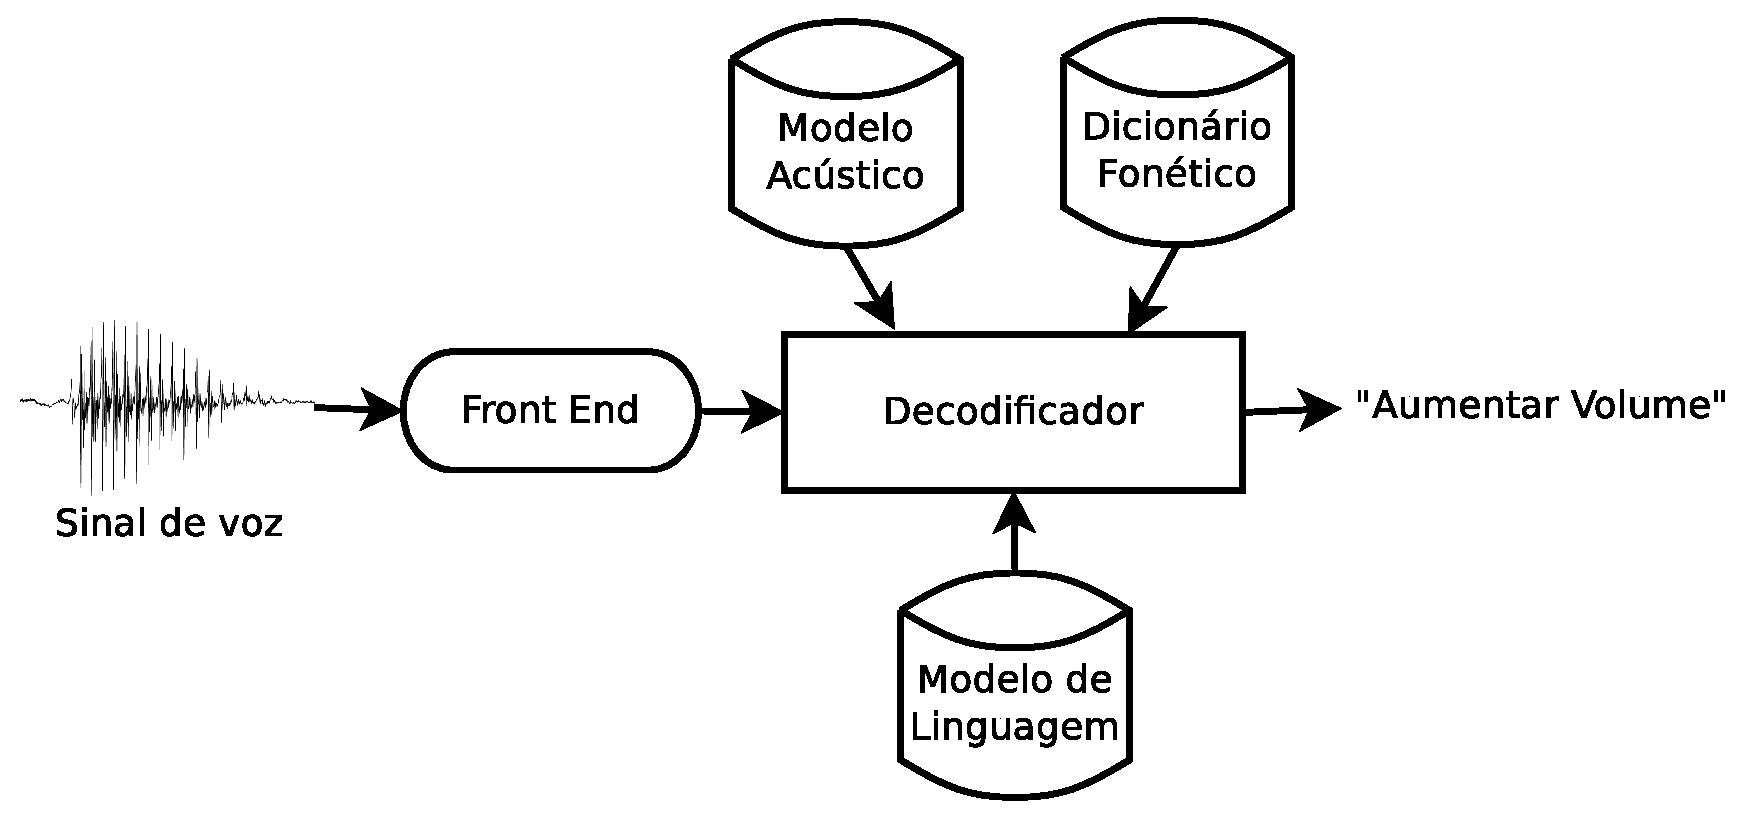
\includegraphics[width=.65\textwidth]{Figures/asr_sch}
	\caption{Esquem�tico de um sistema ASR}
	\label{fig:asr_sch}
\end{figure}

Os fundamentos do reconhecimento autom�tico de voz, assim como os da s�ntese de
voz, s�o descritos com bastante detalhes em~\cite{Huang01}. A arquitetura mais
geral e aceita na literatura � mostrada na Figura~\ref{fig:asr_sch}. Vale
salientar que, ao inv�s do uso de modelos mais gerais, que descrevem a maior
parte de uma linguagem, ser�o utilizadas gram�ticas livres de contexto, as quais
limitam o vocabul�rio utilizado a apenas um conjunto de senten�as poss�veis,
escolhidas pelo desenvolvedor do sistema. A constru��o do dicion�rio fon�tico
para PT\_BR dar-se-� atrav�s do software descrito em~\cite{Siravenha08}; o
tutorial para o treino do modelo ac�stico encontra-se dispon�vel na p�gina do
projeto Voxforge~\cite{voxforge}, bem como cap�tulo 3 do livro do
HTK~\cite[p.~22--42]{Young00}; a gram�tica reconhecida pelo Julius � criada
manualmente de acordo com o descrito na p�gina oficial~\cite{juliussite}.
Instru��es de configura��o e utiliza��o do Julius encontram-se na documenta��o
oficial~\cite{julius_book}.

%\begin{figure}[!h]
%	\centering
%	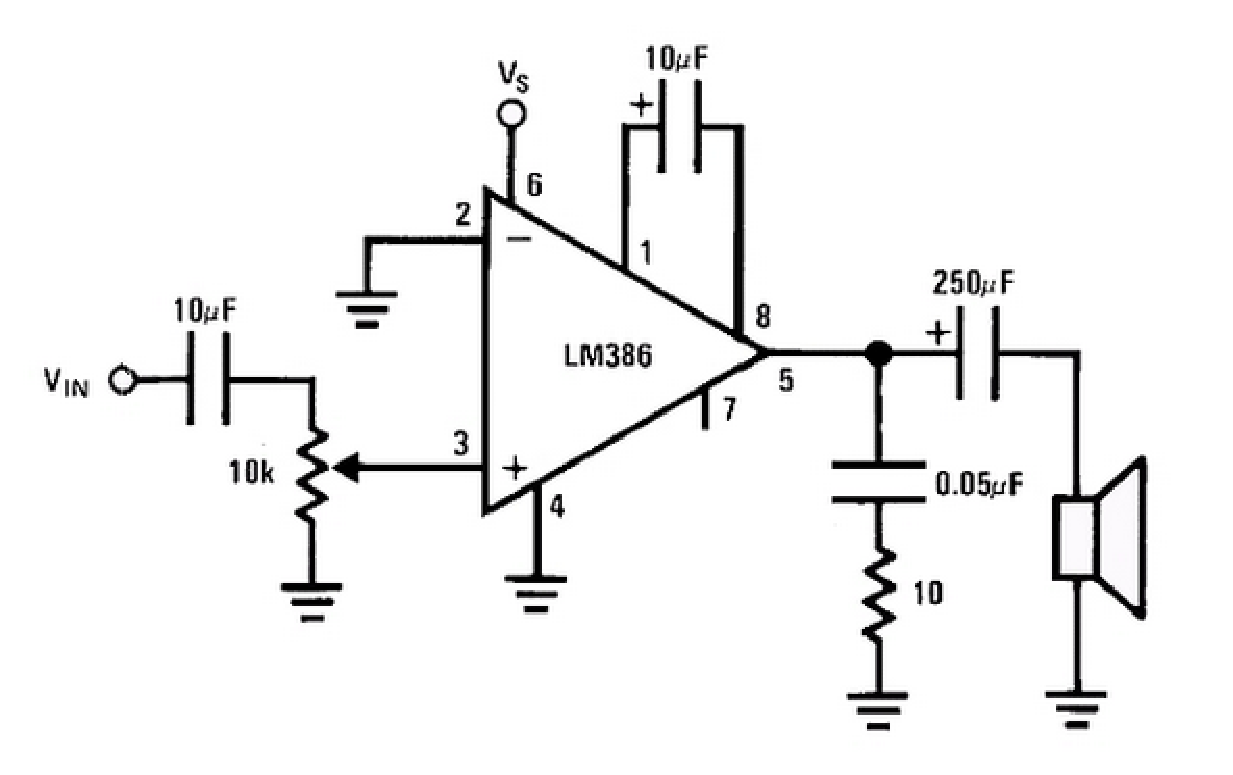
\includegraphics[width=.6\textwidth]{Figures/soundcard_sch}
%	\caption{Esquem�tico de um circuito com auto-falante utilizando o
%	amplificador LM386.}
%	\label{fig:sc_sch}
%\end{figure}

% http://andicelabs.com/2014/03/usb-audio-beaglebone/
Como sa�da anal�gica do sistema TTS, a voz sintetizada deve ser reproduzida por
um dispositivo externo � BeagleBone, j� que esta n�o possui auto-falantes
pr�prios. Como visto em~\cite{andicelabs}, o dispositivo prim�rio de sa�da de
�udio da BeagleBone � o HDMI, o qual pode ser desabilitado mediante modifica��es
em par�metros do kernel. Feito isso, o USB, que � o dispositivo secund�rio, se
torna o principal, fazendo com que a solu��o mais simples seja plugar um 
auto-falante (\textit{speaker}) na porta USB.
Na p�gina oficial do eSpeak, um arquivo de cabe�alho (\textit{header}) permite a
utiliza��o de uma API em C/C++, a qual facilita o acesso aos m�dulos do software
que permitem que a BeagleBone ``fale''~\cite{eSpeak}.

%% http://arduino.cc/en/Tutorial/SimpleAudioPlayer
%% http://www.instructables.com/id/Simple-Wav-Player-Using-Arduino/?lang=pt&ALLSTEPS
%% http://forum.arduino.cc/index.php?topic=49654.0 -- can arduino talk without shield?
%% http://www.instructables.com/id/Twitter-Enabled-Text-to-Speech/
%Links �teis podem ser encontrados em~\cite{arduino_player}
%e~\cite{instructables_player}, os quais ensinam o passo-a-passo para o projeto e
%constru��o de um circuito amplificador. 

A escolha da plataforma foi fundamental para a esquematiza��o do projeto.
Arduino, Raspberry Pi e BeagleBone Black foram as tr�s principais plataformas a
serem escolhidas. Diversos tutoriais de compara��o entre as plataformas foram
consultados e est�o dispon�veis na Internet~\cite{mhl,randomnerd,makezine}.
O Arduino, apesar de ser uma ferramenta flex�vel e com grande capacidade de
interfaceamento com uma vasta quantidade de dispositivos, � uma plataforma
simples, recomendada para projetos de menor porte. O microcontrolador, que pode 
ser programado em C, se torna muito limitado quando o projeto requer um servidor
est�vel e relativamente potente;
O Raspberry Pi, por ser bastante completo, pode ser considerado um mini 
computador. Todo o seu armazenamento � fornecido por um cart�o SD, al�m de ser
poss�vel conect�-lo � Internet atrav�s de um conector Ethernet. Sendo
necess�rio a instala��o de um sistema operacional, o Raspberry Pi ainda possui
interface de sa�da HDMI e � muito �til para aplica��es gr�ficas.

\begin{table}[!h]
\centering
\caption{Compara��o entre as tr�s principais plataformas}
\label{comparison}
\begin{tabular}{c|c c c}
\hline
				& Arduino UNO & BeagleBone Black & Raspberry Pi \\
\hline
Chip			& - & TI AM3359 & BCM2835 SoC full HD \\
CPU				& 20 MHz ATMega328 & 1 GHz ARM Cortex-A8 & 700 MHz ARM1176JZ-F \\
GPU				& - & PowerVR SGX530 & Dual Core VideoCore IV \\
Armazenamento	& 2 kB SRAM & 512 MB DDR3 & 512 MB SDRAM\\
Flash			& 32 kB & 2 GB eMMC, MicroSD & SD, MMC, SDIO card slot\\
GPIO			& 14 & 65 & 8 \\
Video			& - & mini HDMI & HDMI\\
OS				& - & Linux & Linux \\
Amperagem (mA)	& 42 & 210-460 & 150-350 \\
Voltagem (V)	& 7-12 & 5 & 5 \\
USB				& - & 1 Host, 1 Mini Client  & 2 Hosts, 1 Micro Power\\
Ethernet		& - & 1 10/100 Mbps & 1 10/100 Mbps \\
Pre�o 			& 5 conto & 300 conto & 200 conto \\
%Resolu��o		& - & 1280x1024 (5:4), 1024x768 (4:3), 1280x720 (16:9), 1440x900 (16:10) all at 16 bit	& 	Extensive from 640x350 up to 1920x1200, this includes 1080p\\
%Camera connector & - & - & Rpi \\
\hline
\end{tabular}
\end{table}

A BeagleBone � compar�vel ao Raspberry Pi. Entretanto, por ter mais pinos
(GPIO) e um processador mais poderoso, a BeagleBone � uma escolha �bvia para
projetos mais elaborados. Al�m de possuir diversas op��es de conex�o, a
BeagleBone une a flexibilidade de interfaceamento do Arduino com a capacidade
de processamento r�pido do Raspberry Pi. Apesar da desvantagem no pre�o, n�o
restaram muitas d�vidas no momento da escolha dessa plataforma para o projeto.
Uma compara��o entre os principais par�metros dos tr�s equipamentos � dada na
Tabela~\ref{comparison}.

%O cliente Android foi criado tamb�m em~\cite{cassio14}. A interface ser�
%redefinida e m�todos ser�o criados para que haja intera��o com o banco de dados
%a ser instalado no servidor BeagleBone, o qual ficar� encarregado de armazenar
%os dados relacionados � diferentes modelos ou fabricantes de televisores.

O funcionamento de controles remotos, com �nfase nos baseados em luz
infravermelha para televisores, � explicado de de forma clara e detalhada em
diversos tutoriais para ``curiosos'' dispon�veis na Internet, como os da revista
Mundo Estranho~\cite{mundoestranho} e do blog \textit{How Stuff Works?} da
UOL~\cite{uol_hsw}. A maioria dos aparelhos eletr�nicos atualmente recebe
informa��o atrav�s de sensores infravermelhos localizados em pain�is frontais.
Um grande problema � a intefer�ncia que surge com a vasta transfer�ncia de
informa��o via IR. Devido � isso, a comunica��o entre o controle remoto e a
televis�o ocorre em 4 passos: um comando \textit{start} inicia a transfer�ncia,
seguido dos bits do comando espec�fico (como aumentar o volume, por exemplo) e
do endere�o do aparelho. Por fim, um comando de \textit{stop} encerra o envio de
bits. Dessa forma, a chance de a informa��o ser reconhecida por mais de um
aparelho � baixa (salvo o caso de serem dois equipamentos do mesmo tipo e da
mesma empresa).

\subsection{Produtos Relacionados}
Existe uma s�rie de produtos dispon�veis no mercado com a finalidade de tornar o
controle de equipamentos eletr�nicos mais pr�tico. 
Harmony Smart Control\\
\end{section}
%%% EOF %%%


% Metodologia ------------------------------------------------------------------
\begin{section}{Metodologia}
\subsection{Prepara��o do Servidor}
O servidor, por ser o elemento chave na consolida��o do projeto, deve ser o 
m�dulo a ser prioritariamente configurado, a fim de ser preparado para atender
�s devidas requisi��es, bem como executar qualquer tipo de aplica��o solicitada.
Sendo assim, a instala��o da plataforma �ngstr\"{o}m foi tomada como o primeiro
passo. �ngstr\"{o}m~\cite{angstrom} � um sistema operacional, baseado em Linux,
preparado exclusivamente para plataformas embarcadas, sendo o padr�o para a 
pr�pria BeagleBone.

\subsection{Reconhecimento de Voz}
% http://eda.eme.ro/handle/10598/28187
Em~\cite{cassio14}, o Julius foi configurado para funcionar em modo servidor
atrav�s da op��o nativa ``-adinnet'' (A/D \textit{Input from Network}, convers�o 
A/D com entrada pela rede). Isso permite que o Julius receba amostras de �udio
via \textit{streaming} atrav�s de uma comunica��o com um cliente gen�rico via
\textit{socket}.

\subsection{S�ntese de Voz}
% http://stackoverflow.com/questions/2661129/espeak-sapi-dll-usage-on-windows

\subsection{Servidor LAMP}

\subsection{Cliente Android}
Tamb�m em~\cite{cassio14}, 

\begin{figure}[!h]
	\centering
	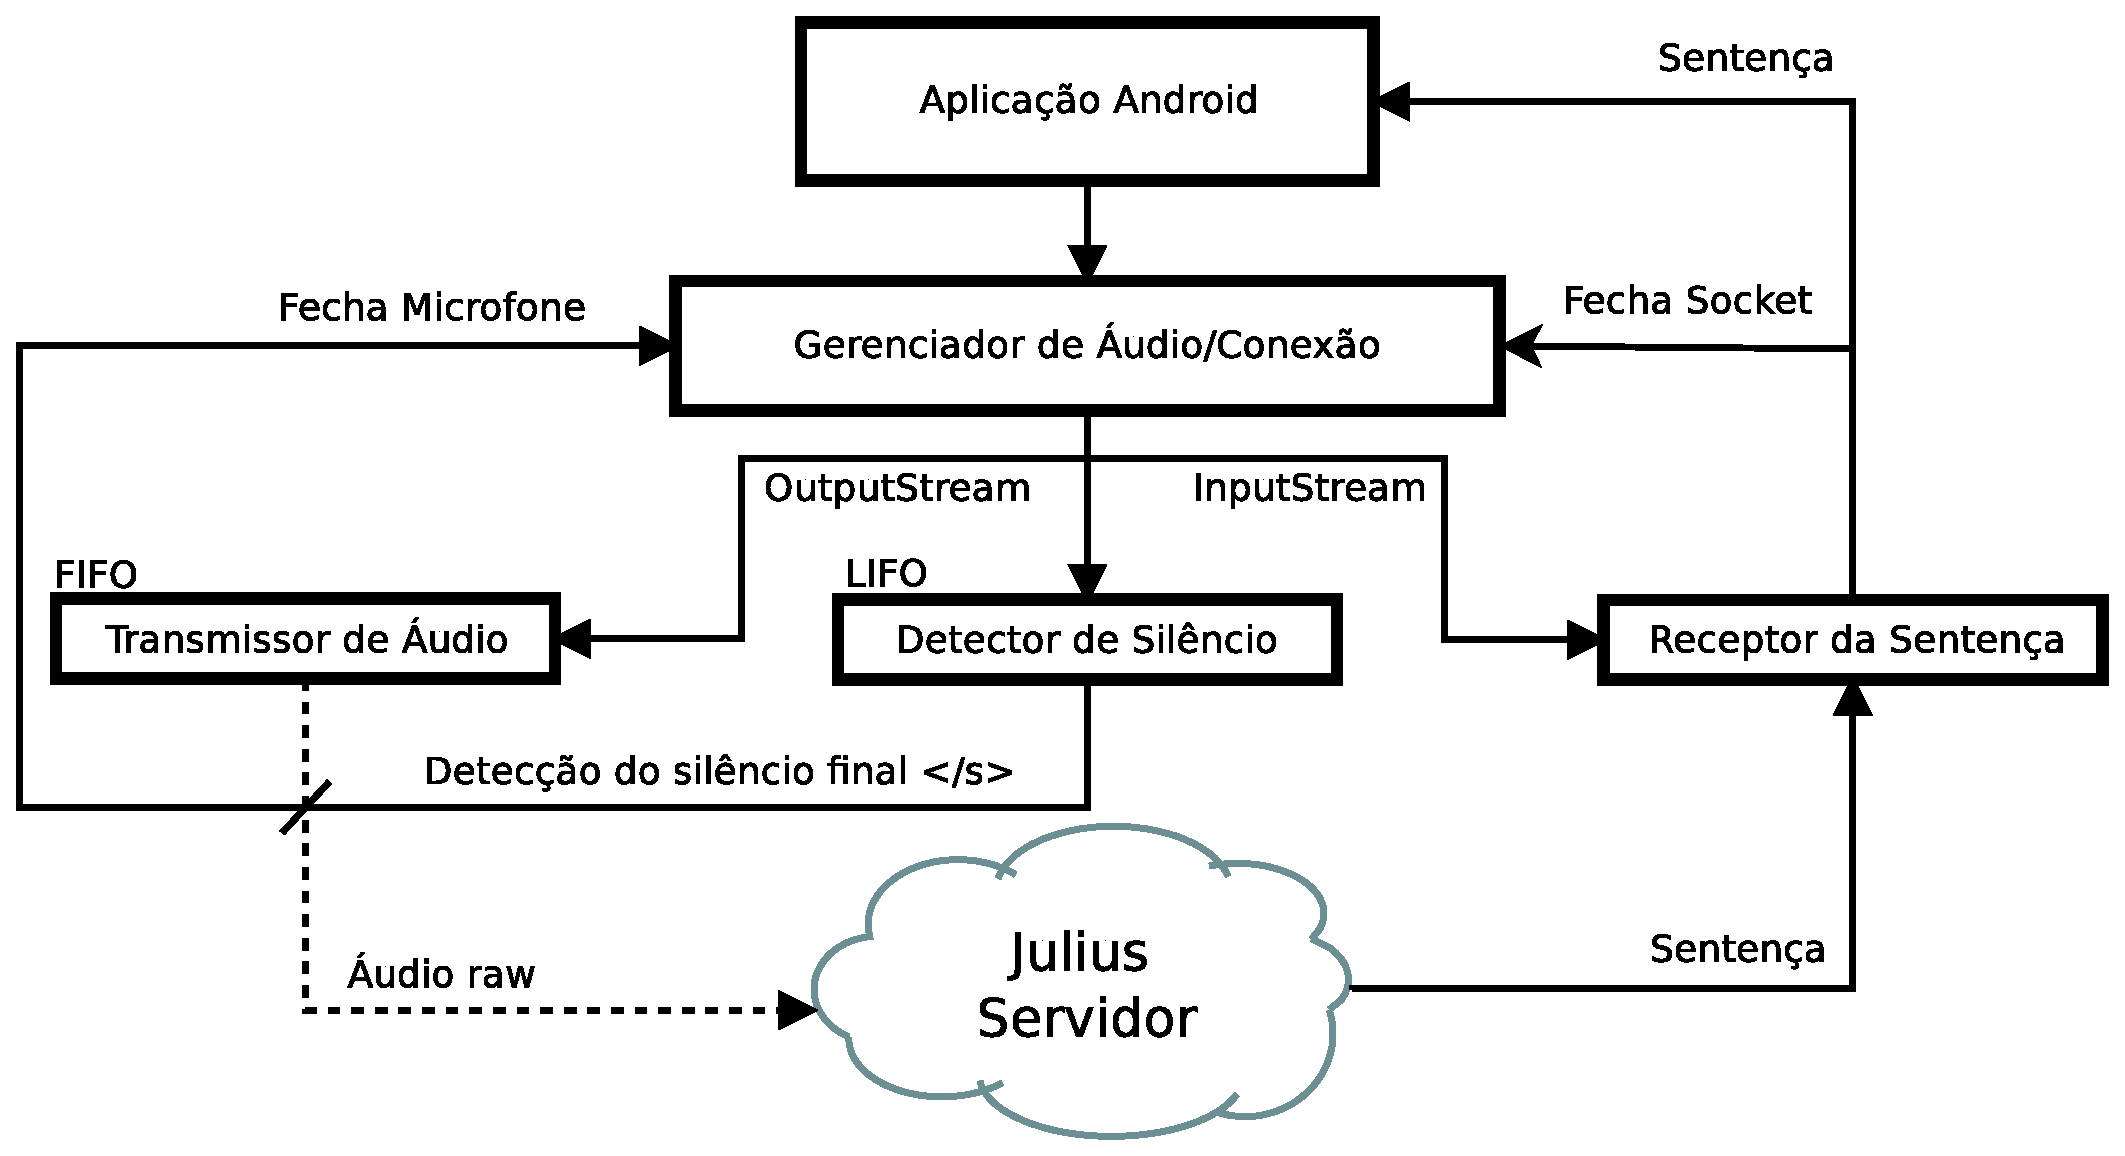
\includegraphics[width=.90\textwidth]{Figures/csr}
	\caption{Esquem�tico do Cliente LaPS CSR.}
	\label{fig:asr_sch}
\end{figure}

\end{section}


% Or�amento --------------------------------------------------------------------
\begin{section}{Or�amento}
% BBB: http://www.farnellnewark.com.br/ : 270,55 + 36,80 = 307,35
% BBB: http://www.aliexpress.com.br/ : 180,34
% Rpi: http://www.aliexpress.com.br/ : 147,92

Aqui � apresentado um or�amento aproximado de todos os materiais utilizados com
base no pre�o de sites de venda online (amazon.com e alibaba.com) e com dados 
recolhidos por Statista em 2013 sobre o pre�o m�dio de smartphones com o sistema
operacional Android. A tabela~\ref{tab:orc} mostra os pre�os de cada material 
juntamente com o total aproximado em d�lar e real.
\begin{table}[!h]
\centering
\caption{Or�amento: Pre�o dos materiais utilizados}
\label{tab:orc}
\begin{tabular}{l|c c c c}
	\hline
	Produto & USD (U\$) & BRL (R\$) & IOF (R\$) & Total (R\$) \\
	\hline
	1 $\times$ BBB & 60.00 & 180.0 & 11.3 & 191.3\\ % Amazon
	1 $\times$ Smartphone & 280.0 & 850.0 & 54.2 & 904.2\\ % Based on data gathered by Statista 2013
	1 $\times$ IR Led (Tx) & 0.10 & 0.30 & 0.02 & 0.32 \\ % 50 = $5
	1 $\times$ IR Receiver (Rx) & 0.14 & 0.42 & 0.03 & 0.45\\ % alibaba.com (LEDs down and above)
	2 $\times$ LEDs (status) & 0.12 & 0.36 & 0.02 & 0.38\\ % 50 = $3
	1 $\times$ USB Headset ANDREA & 40.00 & 120.0 & 7.66 & 127.66\\ % Amazon
	\hline
	Total & 380.36 & 1152.08 & 73.42 & 1225,5\\
\end{tabular}
\end{table}
\end{section}


% Dificuldades e Solu��es ------------------------------------------------------
\begin{section}{Dificuldades e Solu��es}
\begin{enumerate}
\item O �ngstr�m � o sistema operacional de f�brica da BeagleBone, bastante
referenciado em f�runs e candidato principal para ser a base do projeto.
Entretanto, o sistema e a nomenclatura de pacotes n�o correspondiam com os
usados nas distribui��es Debian, o que impossibilitava a instala��o das
depend�ncias necess�rias para o uso das ferramentas de processamento de voz. 
Al�m disso, o �ngstr�m tamb�m consumia muito espa�o de armazenamento na 
\textit{flash}, ocupando sozinho 1.6~GB de 2~GB por conta de sua interface 
gr�fica.

A op��o seguinte foi o Ubuntu, pois a similaridade do sistema de pacotes
\texttt{apt-get} com a distribui��o \textit{desktop} tornaria a integra��o mais
f�cil. Por�m, a instala��o da vers�o 14.04 tamb�m ocupava espa�o demais na
mem�ria \textit{flash}: aproximadamente 1.2~GB. Al�m do problema de espa�o,
outra dificuldade foi a conex�o com a Internet, j� que o acesso convencional ao
reposit�rio de pacotes n�o funcionava. 

A solu��o veio com a instala��o de um terceiro e �ltimo sistema operacional, o 
Debian 7.8 wheezy. Este se mostrou muito mais leve e ``enxuto'' em sua vers�o 
\textit{minimal}, ocupando menos de 500~MB da mem�ria. Al�m disso, todos os 
pacotes necess�rios para conex�o com a Internet funcionaram perfeitamente.

\item A BeagleBone n�o possui sa�da de �udio nativa, tampouco conectores do tipo
\textit{audio jack}. No Debian, a sa�da padr�o de �udio � pelo conector HDMI, 
mas pode ser substitu�da pelo USB mediante modifica��es em par�metros do kernel.
O modo mais f�cil, considerando que redirecionar a sa�da do eSpeak para um GPIO
seria muito trabalhoso, seria conectar um auto-falante USB � BeagleBone. Em se
tratando de um prot�tipo, um \textit{headphone} faz o papel de um
\textit{speaker} que deve consumir pouca energia e ter um tamanho limitado.
Foi-se cogitada a constru��o de um circuito com um amplificador LM386 para o
\textit{speaker}, por�m a obten��o de um D/A PCM2707 n�o custaria menos de 
US\$ 15.

\item A BeagleBone n�o possui conex�o wifi. Al�m da dificuldade em atualizar o
kernel pra receber um \textit{shield/case}, o mesmo teria de ser conectado na 
porta USB, a qual j� estaria sendo usada pelo auto-falante. Portanto, a solu��o
mais f�cil foi conectar um roteador wifi � porta Ethernet da BBB atrav�s de um
cabo UTP.

\item C�digo do Arduino. (Thiago)

\item A fun��o \texttt{mysql\_query()} recebe uma \textit{string} contendo o
comando SQL para acessar o banco de dados MySQL. Caso se queira editar o valor
de um atributo numa determinada tabela, por exemplo, basta passar o valor e o
atributo como par�metros para a fun��o, o que exige que as \textit{strings}
sejam manipuladas constantemente afim de tornar as requisi��es autom�ticas.
Para que n�o se utilize mais espa�os de mem�ria do que necess�rio, optou-se pela
aloca��o din�mica atrav�s da fun��o \texttt{malloc()}, auxiliada pela fun��o
\texttt{sprintf()}, a qual � respons�vel pela jun��o de \textit{strings}. O
c�digo ainda est� sob revis�o, j� que diversas falhas de segmenta��o v�m
ocorrendo devido � erros no gerenciamento de mem�ria. Al�m disso, o custo
computacional provocado pelas diversas \textit{queries} no banco ainda n�o pode
ser previsto. Essa previs�o � muito importante visto que, em uma futura
utiliza��o de um servidor Apache para acesso remoto de qualquer lugar via
cliente PHP, por exemplo, o efeito \textit{snowball} pode surgir como uma
consequ�ncia negativa.

%que usar diversas vezes aloca�\~{o}es de mem\'{o}ria (\textit{*malloc()}) e
%\textit{sprintf()}s, tornando o c\'{o}digo, em mais espec\'{i}fico o
%gerenciamento dos campos da mem\'{o}ria, ca\'{o}tico, apresentando algumas vezes
%falha de segmenta�\~{a}o. Posteriormente, com a adi�\~{a}o de outros aparelhos e
%mais tabelas, estas queries ficaram cada vez mais recorrentes e mais falhas
%poderam acontecer. 

%Al\'{e}m disso, por estarmos acessando o MySQL por meio de uma outra linguagem (no caso C), n\~{a}o podemos prever 
%agora poss\'{i}veis custos computacionais que essas diversas e constantes queries poder\~{a}o gerar nas threads 
%dentro do BeagleBone Black\textregistered. Numa poss\'{i}vel e vindoura utiliza�\~{a}o de um servidor Apache com o 
%PHP essa comunica�\~{a}o adicional e constante poder\'{a} resultar em significante custo computacional tornando-se um 
%efeito \textit{snowball}, bola de neve.
\end{enumerate}
\end{section}
%%% EOF %%%


% Trabalhos Futuros ------------------------------------------------------------
\begin{section}{Trabalhos Futuros}
% http://www.nngroup.com/articles/remote-control-anarchy/
De acordo com o relato dispon�vel em~\cite{nielsen04}: ``Dado que o meu home
theater � modesto, ele requer que eu consiga manejar APENAS 6 controles remotos
para a simples tarefa de assistir a um filme''. Seria marveolous se houvesse um
controle remoto universal que permitisse acesso � TODOS os aparelhos do 
ambiente residencial, mesmo os que est�o em c�modos diferentes do que eu estou
agora. Seria mais maravilhoso que esse controle estivesse sempre com voc�. E que
pudesse us�-lo mesmo quando estivesse fora de casa. E que fosse acess�vel por
uma tecnologia hands free. Compre j� o seu!

\begin{itemize}
	\item Expandir para v�rios aparelhos, tornando a beagle beagle um servidor
	centralizado no ambiente dom�stico
	
	\item Em cada compartimento onde houvesse um aparelho eletr�nico a ser
	controlado, haveria um microcontrolador (a ser avaliado, preferencialmente 
	mais barato que o arduino) capaz de controlar determinado(s) aparelhos

	\item A beagle beagle e todos os outros microcontroladores estariam
	conectados � mesma rede LAN. Somente a beagle beagle precisaria estar
	conectada � internet, de modo que n�o houvesse limita��o de dist�ncia para a
	conex�o com o smartphone.
\end{itemize}
\end{section}
%%% EOF %%%


% Bibliography and References --------------------------------------------------
\bibliographystyle{ieeetr}
\bibliography{tech_report}

% C�digos e Background Matem�tico ----------------------------------------------
\newpage
\appendix
% Pedro ------------------------------------------------------------------------
\begin{section}{C: LAMP}
\label{app:lamp}
Com a sens�vel complexidade dos comandos usados para a comunica��o com a TV
devido ao n�mero de campos e a diferen�a entre eles, foi-se adotado um banco de
ados para armazenar informa��es sobre os aparelhos, bem como seus comandos. Isso
evitar� poss�veis problemas de esvalabilidade quando o sistema evoluir para o
controle de diversos equipamentos eletr�nicos.

% Pedro: o abaixo deveria estar em 'trabalhos futuros'
Al�m disso, visando uma integra��o maior do sistema implementado no BeagleBone
Black$^{\scriptsize{\textregistered}}$, a ado��o de um servidor Apache com PHP 
ser� necess�ria. Essa integra��o se d� pela cria��o de uma p�gina web onde ser�o
armazenados dados provenientes das intera��o do sistema, por exemplo, caso o
usu�rio tenha ligado a TV, mudado de canal ou desligado o ar condicionado, todas 
essas informa��o poder�o ir para um log de uma p�gina web em que pode ser
acessado pelo desenvolvedor para investigar a performance do sistema. Al�m do
log de comandos executados pelo usu�rio, podemos guardar erros cometidos pelo
Julius, ou eSpeak ou ainda falha no envio do comando para o aparelho eletr�nico,
em casos mais espec�ficos o usu�rio poder� at� ligar aparelhos remotamente ou o
desenvolvedor avaliar o desempenho do sistema e identificando problemas antes de
uma visita t�cnica. 

Para integrar todos estes recursos � necess�rio um sistema operacional que, no
caso, � um Linux Debian, configurando assim o servidor LAMP (Linux,
Apache HTTP Server, MySQL e PHP). Ap�s a instala��o das depend�ncias e
subsequente configura��o, o acesso e comunica��o com o MySQL via c�digos em C
foi necess�rio. Para tal, a biblioteca \texttt{mysql.h} � usada. No c�digo em C
para a comunica��o, foram criadas 8 fun��es espec�ficas, sendo elas mostradas na
Lista~\ref{lst:dbphi0}.

% Code
\lstinputlisting[style=code, language=c, firstline=9, lastline=22,
caption={Functions Definitions}, label={lst:dbphi0}]
{codes/db_phi.c}

A Lista~\ref{lst:dbphi1} mostra a fun��o main, onde a conex�o com o banco de 
dados � dada pela fun��o \texttt{mysql\_init()}. J� a fun��o \texttt{create\_db()} 
cria um banco chamado \textit{y} com o usu�rio \textit{root}. Depois, a tabela 
\textit{tv} (\texttt{create\_table()}) � criada e logo ap�s os atributos 
v�o sendo inseridos (\texttt{insert\_table()}). Com \texttt{insert\_element()}
atribuimos um valor a um atributo espec�fico e usamos \texttt{get\_element()}
para retirar da tabela o valor de um atributo, que no caso � \textit{volume+} da
marca LG.

% Code
\lstinputlisting[style=code, language=c, firstline=24, lastline=56, 
caption={Main}, label={lst:dbphi1}]
{codes/db_phi.c}

A Lista~\ref{lst:dbphi2} mostra a fun��o respons�vel por fazer a \textit{query} 
no banco de dados. Ela retornar� o valor do atributo espec�fico que se deseja 
obter, recebendo como par�metros a coluna e a marca, bem como a conex�o com o 
MySQL. Com isso,
pode-se selecionar o atributo \textit{column} onde a marca � igual ao
\textit{target} passado � fun��o. Feito isso, a fun��o \texttt{mysql\_fetch\_row()}
� chamada para retornar todos os valores que satisfazem a condi��o exigida pela 
\textit{query}, o qual, para esse caso especifico, ser� um valor �nico.

% Code
\lstinputlisting[style=code, language=c, firstline=58, lastline=98, 
caption={Fun��o \texttt{get\_element()}}, label={lst:dbphi2}]
{codes/db_phi.c}

A fun��o que assinala um valor um atributo da tabela � mostrada na
Lista~\ref{lst:dbphi3}. Os par�metros ir�o montar a sintaxe da \textit{query}
para que a tabela ``TV'' seja atualizada com o valor equivalente �
\textit{value}, na interse��o linha ``marca'' equivalente � \textit{target} com 
a coluna do comando equivalente � \textit{column}. 

% Code
\lstinputlisting[style=code, language=c, firstline=100, lastline=124, 
caption={fun��o {\tt insert\_element()}}, label={lst:dbphi3}]
{codes/db_phi.c}

A fun��o \texttt{create\_table()}, mostrada na Lista~\ref{lst:dbphi4}, tem como 
finalidade criar as tabelas. Ela recebe o nome da tabela a ser criada
(\textit{table}), o nome do banco de dados onde ela ser� criada (\textit{db}), o
usu�rio (\textit{user}), a senha desse usu�rio (\textit{pwd}) e a conex�o
MySQL (\textit{con}). Ela ir� montar com uma sintaxe pr� definida a tabela
com os atributos \textit{marca, volume+, volume-, canal+, canal-, on, off,
address}.

% Code
\lstinputlisting[style=code, language=c, firstline=154, lastline=187, 
caption={fun��o {\tt create\_table()}}, label={lst:dbphi4}]
{codes/db_phi.c}

A Lista~\ref{lst:dbphi5} mostra a fun��o \texttt{create\_db()}, a qual tem como 
finalidade a cria��o do banco de dados.  O nome do banco a ser criado, o usu�rio
e a senha desse usu�rio s�o passadas como par�metro, bem como e a conex�o com o
MySQL. Ela usa o nome \textit{name} para organizar a sintaxe que cria o banco.

% Code
\lstinputlisting[style=code, language=c, firstline=189, lastline=202,
caption={fun��o {\tt create\_db()}}, label={lst:dbphi5}]
{codes/db_phi.c}

%% Code
%\lstinputlisting[style=code, language=c, firstline=205, lastline=210, 
%caption={fun��o {\tt finish\_with\_error()}}, label={lst:dbphi6}]
%{codes/db_phi.c}
%
%A fun��o \texttt{finish\_with\_error()}, mostrada na Lista~\ref{lst:db_6}, 
%apenas oferece o erro padr�o para o caso de a conex�o MySQL seja executada com
%erro.

%% Pedro: escrota essa fun��o handle n gostei elimine
%Em algumas sintaxes do MySQL os atributos s�o passados como ``nome'', ou seja,
%entre aspas duplas, entretanto para inserir estas aspas duplas em C n�o
%� t�o trivial assim caso queiramos automatizar o processo de
%adi��o, portanto, esta fun��o foi criada com a finalidade
%espec�fica de adicionar e manipular esta string para que ela saia "string".
%Ela recebe apenas a string alvo (no caso \textit{$*user$}, pois o caso onde a
%usamos � para garantir acesso a algum usu�rio ao banco de dados.

%% Pedro: ajeita essa fun��o GRANT no .c e inclui ela da forma que inclu� 
%% as outras a� em cima
%\begin{lstlisting}[style=code, language=c, caption={fun��o $grant\_db()$}, label={lst:dbphi8}]
%int grant_db(char *user, char *db, MYSQL *con){
%    char *grantall = "GRANT ALL ON y.* TO GUEST IDENTIFIED BY ";
%	char *flush_command = "FLUSH PRIVILEGES";
%
%	char *user_handle = handle_string(user);
%
%	size_t grant_len = strlen(grantall)+strlen(user_handle);
%
%	char *grant_command = (char *) malloc((grant_len+1)* sizeof (char));
%
%	sprintf(grant_command, "%s%s", grantall,user_handle);
%
%	printf("user_handle = %s\n",user_handle);
%	printf("%s\n",grant_command);
%
%	if(mysql_query(con, "GRANT ALL ON y TO GUEST IDENTIFIED BY \"phy_dev\""))
%		finish_with_error(con);
%
%	printf("Grant Success!\n");
%	
%	if(mysql_query(con,"FLUSH PRIVILEGES"))
%		finish_with_error(con);
%
%	free(result);
%	free(grant_command);	
%	exit(0);
%}
%\end{lstlisting}
%
%Aqui garantimos ao usu�rio \textit{$*user$} acesso ao banco de dados
%\textit{$*db$}, por meio de uma conex�o MySQL \textit{$*con$}. Nela usamos a
%fun��o \textit{$handle\_user()$} para modificar a string do usu�rio
%e posteriormente us�-la para montar a sintaxe da \textit{query}.
\end{section}

% Thiago -----------------------------------------------------------------------
\newpage
\begin{section}{Arduino: IR Tx/Rx}
\label{app:arduino}
\lstinputlisting[style=code, language=c, firstline=12, lastline=26,
caption={Declara��es globais}, label={lst:ard_1}]
{codes/arduino_IR.ino}

\lstinputlisting[style=code, language=c, firstline=34, lastline=68,
caption={Fun��o {\tt loop()}}, label={lst:ard_2}]
{codes/arduino_IR.ino}

\lstinputlisting[style=code, language=c, firstline=70, lastline=83,
caption={Fun��o {\tt printPulses()}}, label={lst:ard_3}]
{codes/arduino_IR.ino}

\lstinputlisting[style=code, language=c, firstline=85, lastline=99,
caption={Fun��o {\tt pulseIR()}}, label={lst:ard_4}]
{codes/arduino_IR.ino}

\lstinputlisting[style=code, language=c, firstline=101, lastline=108,
caption={Fun��o {\tt sendCommand()}}, label={lst:ard_5}]
{codes/arduino_IR.ino}
\end{section}

% Cassio -----------------------------------------------------------------------
\newpage
\begin{section}{Matlab/Octave: Analisador de Onda Quadrada}
\label{app:matlab}
\lstinputlisting[style=code, language=matlab]{codes/myanalyze.m}
\end{section}

% Cassio -----------------------------------------------------------------------
\newpage
\begin{section}{C: RC-6 \textit{Handler}}
\label{app:rc6}
\lstinputlisting[style=code, language=c, firstline=57, lastline=67,
caption={Declara��o das fun��es}, label={lst:ir_0}]
{codes/ir_pwm.c}

\lstinputlisting[style=code, language=c, firstline=133, lastline=211,
caption={Fun��o \texttt{decode()}}, label={lst:ir_1}]
{codes/ir_pwm.c}

\lstinputlisting[style=code, language=c, firstline=220, lastline=278,
caption={Fun��o \texttt{send()}}, label={lst:ir_1}]
{codes/ir_pwm.c}

\lstinputlisting[style=code, language=c, firstline=281, lastline=323,
caption={Fun��o \texttt{receive()}}, label={lst:ir_1}]
{codes/ir_pwm.c}
\end{section}
%%% EOF %%%

\end{document}
%%% EOF %%%
